\chapter[Setup der Experimente (Schmelzer)]{Setup der Experimente}

Der SegMap-Algorithmus ist aus mehreren ROS-Paketen aufgebaut. 
%Dies ist ein Open Source Framework, das verschiedene Bibliotheken und Werkzeuge für die Entwicklung von Roboteranwendungen umfasst. Es bietet beispielsweise verschiedene Gerätetreiber und Visualisierungswerkzeuge sowie ein eigenes System zum Austausch von Nachrichten zwischen verschiedenen Prozessen.
%https://www.ros.org/
Um den Algorithmus für die Anwendung auf RGB-D Daten in einer indoor-Umgebung validieren zu können, werden indoor-Datensätze benötigt, die RGB-D Daten und Odometrieinformationen enthalten. Diese müssen in einer ROS-kompatiblen Form vorliegen. Hierfür wird der Nachrichten-Stream der verschiedenen Sensoren in von ROS definierten Sensornachrichtenformaten mit zugehörigem Zeitstempel in Bag-Dateien gespeichert. 

Es gibt viele verschiedene frei verfügbare indoor RGB-D Datensätze, bei denen z.B. diverse Räume statisch mit einer RGB-D Kamera aufgenommen wurden. Die Daten müssen allerdings als Stream kontinuierlich aufeinander folgender Nachrichten in einem ROS-Sensornachrichtenformat zur Verfügung stehen. Es handelt sich um einen SLAM-Algorithmus bei dem die Trajektorie des Roboters sowie die entstehende Karte der Umgebung laufend durch die Erkennung von Loop Closures korrigiert werden. Daher muss der Datensatz für eine sinnvolle Validierung auch Schleifen enthalten, bei denen Teile der Umgebung mehrmals besucht werden. Eine Umwandlung der öffentlich zugänglichen Datensätze auf die genannten Anforderungen  ist sehr aufwendig. Daher wurden für die Validierung eigene Datensätze erstellt. 

Im Folgenden wird die verwendete Hardware für die Erstellung der Datensätze sowie die Ausstattung des für die Validierung des Algotihmus verwendeten Computers vorgestellt. Außerdem werden die Datensätze anhand derer die Validierung durchgeführt wird präsentiert und erläutert wie diese erstellt wurden.

\section[Kamera (Kopp)]{Kamera}
\label{sec:kamera}

Es gibt auf dem Markt viele verschiedene RGB-D Kameras. Diese unterscheiden sich typischerweise neben den Preisen, der Verfügbarkeit und ihrer physikalischen Dimensionen auch hinsichtlich des Blickwinkels, der Auflösung und der Reichweite. Außerdem werden Hersteller-abhängig unterschiedliche APIs geliefert, die sich hinsichtlich der Anwenderfreundlichkeit und der Hard- und Software-spezifischen Anforderungen zur Systemintegration unterscheiden. 

Für die Auswahl einer geeigneten Kamera für die Aufnahme der Datensätze wurden einige Kriterien aufgestellt, die von der Kamera erfüllt werden müssen. 

\subsection[Kriterien (Kopp)]{Kriterien}

Da indoor-Umgebungen sich in der Regel nicht über große Entfernungen erstrecken, ist die Sichtweite recht beschränkt. Daher wird als relevanter Bereich für eine Orientierung in solchen Umgebungen ein Messbereich von bis zu 10 m Entfernung zum Sensor definiert. Die Reichweite der Kamera sollte etwa diese Entfernung abdecken. 

Der SegMap-Algorithmus ist auf die Verarbeitung der Daten eines hochauflösenden LiDAR-Sensors ausgelegt. Als relevanter Bereich für die Datenverarbeitung wurden 50 m gewählt. Die Validierung erfolgte anhand des KITTI-Odometrie Datensatzes. Zur Punktwolkenerzeugung wird dabei ein Velodyne HDL-64E Laserscanner verwendet. Um ähnlich gute Ergebnisse  zu erzielen, sollte die Kamera in der definierten maximalen Distanz von etwa 10 m über eine ähnlich gute Auflösung wie dieser, bezogen auf die geometrische Beschaffenheit der Umgebung, verfügen.

Die horizontale Auflösung des verwendeten Velodyne Scanners beträgt laut Datenblatt 0,08$^\circ$ die vertikale Auflösung 0.4$^\circ$. Wie bereits erwähnt, ist im Außenbereich eine Umgebung von bis zu 50 m Entfernung von Interesse. Um eine Vergleichbarkeit zu schaffen, muss die Auflösung auf die relevanten Entfernungen bezogen berechnet werden. Wie auf Abbildung \ref{fig:Auflösung} dargestellt, kann der Abstand $a_d$ zweier Punkte anhand der Entfernung $d$ zum Sensor und dem Winkel $\alpha$, der dem gegeben Winkel der Auflösung entspricht, berechnet werden. Hierfür wird folgende Formel verwendet:

\begin{align}
	a_d= d*sin(\alpha)/cos(\alpha)
\end{align}

Mit der gegebenen Auflösung und einer maximalen Entfernung von 50 m, ergibt sich somit ein horizontaler Punktabstand von $\sim$7 cm. In vertikaler Richtung beträgt der Punktabstand entsprechend $\sim$ 35 cm. Ein etwa 2$\times$2 m messende Fläche in 50 m Entfernung kann somit durch circa 140 Punkte repräsentiert werden. Damit wird es als Segment in die Karte geschrieben, da hierfür eine Begrenzung von mindestens 100 Punkten gesetzt ist. 

\begin{figure}
	\centering
	\includegraphics[width=0.5\linewidth]{Bilder/Aufloesung_Kamera_LIDAR.png}
	\caption{Darstellung der Auflösung anhand des Punktabstandes in einer definierten Entfernung d}
	\label{fig:Auflösung}
\end{figure}

Betrachtet man Strukturen, die im Innenbereich potentielle Segmente darstellen können, so stellen Türen, Tische, Schränke, Fenster oder auch ein hervorstehender Lichtschalter potentielle Kandidaten dar. Daraus abgeleitet ergibt sich das Kriterium Strukturen mit Kantenlängen ab 10$\times$10 cm in einer Entfernung ab 50 cm genügend Punkte für eine Segmentierung zuordnen zu können. Auf eine Entfernung von 10 m sollten Türen und Schränke noch sicher Segmente ergeben. 

Zusätzlich sollte es für die Kamera eine ROS-Anbindung geben, um eine einfache Generierung der Daten im benötigten ROS-Sensornachrichtenformat zu ermöglichen. Außerdem sollte eine Framerate von 10 Hz erreicht werden und die Kamera einfach auf dem Markt verfügbar sein. 

%Da der SegMap-Algorithmus mit LiDAR Daten arbeitet, erfolgt eine Gegenüberstellung der erreichten Auflösung der jeweiligen Systeme. Dabei ist zu berücksichtigen in welcher Entfernung die jeweiligen Sensoren relevante Informationen aufnehmen. Im Außenbereich beträgt dieser relevante Bereich zwischen 3 m und 50 m Entfernung. Für den Innenbereich wird definiert, dass zwischen 0,5 m und 10 m der relevante Messbereich liegt. Die Auflösung im Innenbereich sollte in der formulierten Distanz ausreichend hoch gewählt werden, um Segmente anhand der geometrischen Beschaffenheit der Umgebung zu erzeugen.

%Die Verfasser des SegMap Algorithmus verwenden in ihren Experimenten den KITTI Odometrie Datensatz. Zur Punktwolkenerzeugung wird dabei ein Velodyne HDL-64E Laserscanner verwendet. Die Auflösungen der jeweiligen Sensoren müssen einmal in horizontaler und einmal in vertikaler Auflösung verglichen werden. Die horizontale Auflösung des Velodyne Scanners beträgt laut Datenblatt $0,08^\circ$ die vertikale Auflösung $0.4^\circ$. Wie bereits erwähnt, ist im Außenbereich eine Umgebung von 3-50 m von Interesse. Um eine Vergleichbarkeit zu schaffen, muss die Auflösung auf die relevanten Entfernungen bezogen berechnet werden. $a_d$ steht dabei für den Abstand zweier Punkte in einer Entfernung $d$, siehe Abbildung \ref{fig:Auflösung}. Mit dem gegebenen Winkel $\alpha$ und einer Entfernung von 50 m ergibt sich mit $ a_d= d*sin(\alpha)/cos(\alpha)$ ein Punktabstand von $\backsim$ 7 cm bei $d$ = 10m von $\backsim$ 1,4cm. Die horizontale Auflösung in 10 Metern beträgt $\backsim$ 7 cm, in 50m Entfernung $\backsim$ 35cm. Ein etwa $2 \times 2$m  messendes Objekt in 10 m Entfernung kann somit durch ca. 4000 Punkte repräsentiert werden.  In einer Entfernung von 50 m erzeugt die gleiche Fläche ca. 140 Punkte. Ein Segment wird ab einer Mindestpunktzahl von 100 Punkten als solches verarbeitet, die maximale Punktzahl beträgt 15000 Punkte. Betrachtet man Strukturen die im Innenbereich potentielle Segmente darstellen können, so stellen Türen, Tische, Schränke, Fenster oder auch ein hervorstehender Lichtschalter potentielle Kandidaten dar. Daraus abgeleitet entstand das Kriterium Strukturen mit Kantenlängen ab $10\times 10$cm in einer Entfernung ab 50 cm genügend Punkte für eine Segmentierung zuordenen zu können. Auf eine Entfernung von 10 m sollten Türen und Fenster noch sicher Segmente ergeben. Die auf dem Markt erhältlichen Kameramodelle, die in der folgenden Tabelle aufgeführt sind, werden auf deren Auflösung, Preis, Framerate, Verfügbarkeit, Baugröße, Bildausschnitt und Typ  hin geprüft.


\subsection[Intel Realsense D435 (Kopp)]{Intel Realsense D435}

In Tabelle \ref{tab:Kameras} sind die technischen Eigenschaften einiger auf dem Markt erhältlichen Kameramodelle aufgeführt. Sie verfügen alle über eine ROS-Anbindung und liefern zusätzlich zu den Tiefeninformationen ein Farbbild. Hinsichtlich der genannten Kriterien werden die verschiedenen Kameras geprüft, ob diese erfüllt werden. Außerdem werden die Preise sowie die Baugröße verglichen. In der Tabelle beschreibt FOV das Sichtfeld, das in horizontaler und vertikaler Richtung abgedeckt wird. 

%Die auf dem Markt erhältlichen Kameramodelle, die in der folgenden Tabelle aufgeführt sind, werden auf deren Auflösung, Preis, Framerate, Verfügbarkeit, Baugröße, Bildausschnitt und Typ  hin geprüft.

\begin {table}[th!]
\setlength{\tabcolsep}{0.6mm}
\begin{tiny}
 \centering
 \caption{Technische Daten verschiedener RGB-D Kameras mit ROS-Anbindung \cite{ROSIND2020}}
 \label{tab:Kameras}
 \begin{tabulary}{\textwidth}{ L C C C C C C C C }
  \hhline{=========}
    Kamera & Typ & Reichweite (m) & 3D-Auflösung & RGB-Auflösung & Framerrate (fps) & FOV & Abmessungen (mm) & Preis (Euro)\\
  \hhline{=========}
  Microsoft® Kinect™ 2.0 & Time of flight & 0.5-4.5 & 512$\times$424 & 192$\times$1080 & 30 & 70$^\circ$H, 60$^\circ$V & 250$\times$70$\times$45 & 149  \\
  \hhline{---------}
  ASUS® XtionPro™ Live & Structured Light &  0.8-3.5 & 640$\times$480 & 1280$\times$1024 & 30 & 58$^\circ$H, 45$^\circ$V & 180$\times$40$\times$25 & - \\
  \hhline{---------}
  Stereolabs® ZED™& Embedded Stereo & 1.5-20 & 2208$\times$1242 & 2208$\times$1242 & 15-120 & 96$^\circ$H, 54$^\circ$V & 175$\times$30$\times$33 & 349 \\
  \hhline{---------}
  CarnegieRobotics® MultiSense™ S7 & Embedded Stereo & 0.4m-$\infty$ & 2048$\times$1088 & 2048$\times$1088 & 15 & 80$^\circ$H, 45$^\circ$V & 130$\times$130$\times$65 & - \\
  \hhline{---------}
  Ensenso® N35-606-16-BL & Structured Light & - & 1280$\times$1024 & 1280$\times$1024 & 10 & 58$^\circ$H, 52$^\circ$V & 175$\times$50$\times$52 & - \\
  \hhline{---------}
  Nerian SceneScan & FPGA Stereo Camera & - & 1856$\times$1856 & 1856$\times$1856 & 100 & - & 144$\times$41$\times$35mm & - \\
  \hhline{---------}
  Intel® RealSense™ Camera D415 & Active IR Stereo & 0.3-10 & 1280$\times$720 & 1920$\times$1080 & 30-90 & 63.4$^\circ$H, 40.4$^\circ$V & 99$\times$20$\times$23 & 167 \\
  \hhline{---------}
  Intel® RealSense™ Camera D435 & Active IR Stereo & 0.105-10 & 1280$\times$720 & 1920$\times$1080 & 30-90 & 85.2$^\circ$H, 58$^\circ$V & 99$\times$25$\times$25 & 200 \\
  \hhline{---------}
  FRAMOS Depth Camera D435e & Active IR Stereo & 0.2-10 & 1280$\times$720 & 1920$\times$1080 & 30 & 86$^\circ$H, 57$^\circ$V & - & - \\
  \hhline{---------}
  Orbbec® Astra Mini™ & Structured Light & 0.6-5 & 640$\times$480 & 640$\times$480 & 30 & 60$^\circ$H, 49.5$^\circ$V & 80$\times$20$\times$20 & 185 \\
  \hhline{---------}
  Arcure Omega & Stereo & 0.3-50 & 1280$\times$1024 & 1280$\times$1024 & 60 & 120$^\circ$H, 90$^\circ$V & 200$\times$83$\times$79 & - \\
   \hhline{=========}
\end{tabulary}
\end{tiny}
\end{table}
%
%\begin{table}
%\label{tab:Kameras}
%	\caption{Technische Daten verschiedener RGB-D Kameras mit Ros-Anbindung}
%\begin{flushleft}
%\begin{tiny}
%\setlength{\tabcolsep}{0.6mm}
%\begin{tabular}[h]{@{}p{3cm}|p{1,5cm}|c|c|c|c|c|c|c|}
%Kamera&Typ&Reichweite&3D Auflösung&RGB Auflösung&Framerrate&FOV & Abmessungen &  Preis \\
%\hline
%Microsoft® Kinect™ 2.0 & Time of flight&0.5-4.5m&512x424&1920x1080&30fps&70$^\circ$H,60$^\circ$V&250x70x45mm&149  \\
%\hline
%ASUS® XtionPro™ Live & Structured light&0.8-3.5m&640x480&1280x1024&30fps&58$^\circ$H,45$^\circ$V& 180x40x25mm&-  \\
%\hline
%Stereolabs® ZED™& Embedded stereo&1.5-20m&2208x1242&2208x1242&15-120 fps&96$^\circ$H,54$^\circ$V& 175x30x33mm& 349 \\
%\hline
%CarnegieRobotics® MultiSense™ S7&Embedded stereo&0.4m-$\infty$ &2048x1088&2048x1088&15 fps&80$^\circ$H,45$^\circ$V&130x130x65 mm & -  \\
%\hline
%Ensenso® N35-606-16-BL & Structured light&-&1280x1024&1280x1024&10fps&58$^\circ$H,52$^\circ$V&175x50x52mm&- \\
%\hline
%Nerian SceneScan&FPGA Stereo Camera&-&1856x1856&1856x1856&100fps&-&144x41x35mm&-  \\
%\hline
%Intel® RealSense™ Camera D415&Active IR Stereo&0.3-10m&1280x720&1920x1080&30-90fps&63.4$^\circ$H,40.4$^\circ$V&99x20x23mm&167  \\
% \hline
%Intel® RealSense™ Camera D435&Active IR Stereo&0.105-10m&1280x720&1920x1080&30-90fps&85.2$^\circ$H,58$^\circ$V& 99x25x25mm&200  \\
% \hline
%FRAMOS Depth Camera D435e&Active IR Stereo&0.2-10m&1280x720&1920x1080&30fps&86$^\circ$H,57$^\circ$V&-&-  \\
% \hline
%Orbbec® Astra Mini™&Structured Light &0.6-5m&640x480&640x480&30fps&60$^\circ$H,49.5$^\circ$V &80x20x20mm&185  \\
% \hline
%Arcure Omega& Stereo&0.3-50m&1280x1024&1280x1024&60fps&120$^\circ$H,90$^\circ$V&200x83x79mm& -  \\
%\end{tabular}
%\end{tiny}
%\end{flushleft}
%\end{table}

Aufgrund des hohen Blickwinkels, der kompakten Bauweise, der schnellen Verfügbarkeit und des niedrigen Preises wird von allen Kameras, die die genannten Kriterien erfüllen, die Realsense D435 der Firma Intel gewählt. Diese nutzt für die Generierung der Punktwolke den Ansatz der aktiven Stereoskopie. Die Auflösung der Punktwolke liegt bei maximal 1280x720 Punkten. Werden nun die gleichen Überlegungen angestellt, wie bei der Analyse des LiDAR-Sensors, ergeben sich bei einer Distanz von 10 m eine horizontale Auflösung von $\sim$15,1 mm und eine vertikale Auflösung von $\sim$14,6 mm. Entsprechend ergeben sich bei einer Entfernung von 0,5 m ein Punktabstand von 0,73 mm in horizontaler und 0,75 mm in vertikaler Richtung. 

Die zuvor angedachte Fläche von 10x10cm in einer Entfernung von 50cm liefern also $\sim$137$\times$133 $\approx$ 23000 Messpunkte. In einer Entfernung von 10 m stehen für eine Fläche von 200x100cm dementsprechend 143$\times$67 $\approx$ 9438 Messpunkte zur Verfügung. Daraus ergibt sich, dass die Auflösung der Kamera hoch genug ist, um typische indoor-Objekte mit der geforderten Punktdichte abzutasten. 

%kommt man bei einer Distanz von 50cm auf eine vertikale Auflösung von $\sim$ 0,73 mm und eine horizontale Auflösung von $\sim$ 0,75mm. Bei einer Entfernung von 10 m beträgt die vertikale Auflösung $\sim$ 14,6 mm, die horizontale Auflösung beträgt $\sim$ 15,1 mm. Die zuvor angedachten 10x10cm in einer Entfernung von 50cm liefern also  $\sim$ 137x133$\approx$ 23000 Messpunkte. In einer Entfernung von 10 m stehen für eine Struktur von 200x100cm dementsprechend 143x67$\approx$9438 Messpunkte zur Verfügung. Aufgrund dieser Berechnung, des günstigen Preises, der kleinen Abmessungen und des geringen Gewichts, aber auch die einfache Integrierung in das ROS Framework, durch bestehende Libraries wurde entschieden diese Kamera zu beziehen.

\subsection[Erweiterung des Sichtfelds (Kopp)]{Erweiterung des Sichtfelds} 
\label{sec:stereo}
 
Im vorherigen Abschnitt wurde erläutert, dass die Punktwolke, die die gewählte RGB-D Kamera erzeugt, ausreichend auflösend ist. Der horizontale Blickwinkel des bei SegMap verwendeten Laserscanners beträgt 360$^\circ$, der Blickwinkel der Kamera jedoch lediglich 85,2$^\circ$. Daher wurde die Überlegung angestellt den Öffnungswinkel zu verbreitern, um die Umgebung besser einfangen zu können. 

Angedacht war die Kamera aktiv durch einen Motor rotieren zu lassen. Die Abbildung \ref{fig:Dreheinheit} zeigt die dafür konstruierte Rotationseinheit. Der horizontale Aufnahmewinkel wird dadurch auf 198$^\circ$ erweitert. Für langsame Bewegungen eines Roboters kann das ein guter Ansatz sein. Bei höherer Geschwindigkeit ist die Gefahr groß Verarbeitungsfehler zu bekommen, da die Bewegungen der Kamera abhängig von der Bewegung der Plattform im Raum sehr genau bestimmt werden muss, um eine konsistente Punktwolke zu generieren.

Eine Alternative stellt eine fixierte Anordnungen von zwei Kameras, wie in Abbildung \ref{fig:Kamera_Starr} zu sehen, dar. Der Winkel zwischen den Kameras wurde so gewählt, dass sich die Punktwolken ab einer Entfernung von 30 cm überlappen. Der Sichtbereich vergrößert sich so auf 158$^\circ$. Die Verarbeitung der Punktwolken durch den fixierten Abstand und Winkel ist sehr viel einfacher als bei einer schwenkbaren Lösung und weniger Fehleranfällig. Anordnungen mit mehr als zwei Kameras wurden nicht in Betracht gezogen, weil die zur Verfügung stehende Hardware für diese Datenmenge nicht ausreichend ist. 

\begin{figure}
	\centering
	\begin {minipage}[t]{0.45\linewidth}
	\centering
	\includegraphics[width=\linewidth]{Bilder/Kameradreheinheit1.png}
	\caption{Darstellung der motorbetriebenen Dreheinheit mit Kamera}
	\label{fig:Dreheinheit}
	\label{fig:Kamera_Starr}
\end{minipage}
\hfill
 \begin{minipage}[t]{0.45\linewidth}
	\centering
	\includegraphics[width=\linewidth]{Bilder/Kamera_Starr.png}
	\caption{Darstellung der starren Anordnung zweier Kameras}
	\label{fig:Kamera_Starr}
\end{minipage}
\end{figure}

Die Sensornachrichten der bei dieser Konfiguration entstehenden Punktwolken werden jeweils in einem Koordinatensystem der aufnehmenden Kamera gepublisht. Mit Hilfe des im ROS-Wrapper der Kamera enthaltenen Python-Skript \textit{set$\_$cams$\_$transform.py} können unter Angabe der relativen Lage der Kameras zueinander die Transformationen zwischen den Kamera-Koordinatensystemen erhalten werden. Anhand dieser Transformationen können die Punktwolken beider Kameras in ein Koordinatensystem übertragen und anschließend als eine Sensornachricht gepublisht werden. Abbildung \ref{fig:stereo} zeigt zum Vergleich zwei Beispiele für die Punktwolke einer Kamera gegen die Punktwolke, die sich aus der Konfiguration mit zwei Kameras ergibt. Das Blickfeld wird deutlich erweitert. 

\begin{figure}
	\centering
	\includegraphics[width=\linewidth]{Bilder/Zwei_vs_eine_Kamera.png}
	\caption{Vergleich der Punktwolke (a) einer einzelnen Kamera und (b) der Punktwolke der Konfiguration mit zwei Kameras }
	\label{fig:stereo}
\end{figure}


\section[Odometrie (Kopp)]{Odometrie}

Der SegMap-Algorithmus benötigt Odometrieinformationen. Die Erzeugung von Odometriedaten einer Roboterplattform kann Hardwareseitig beispielsweise durch Drehgeber an den Achsen oder anhand der Steuerbefehlen geschehen. Außerdem kann Software-basiert, etwa über ICP eine Odometrieschätzung erzeugt werden. Beim SegMap-Algorithmus kann die Trajektorie sowohl anhand Hardware-basierter Odometrieinformtionen als auch durch ICP geschätzt werden. Zusätzlich können beide Verfahren auch fusioniert werden. Jedoch wurde der mitgelieferte ICP-Algorithmus für outdoor-Umgebungen und 360$^\circ$ Rundumsicht parametrisiert. Die Parametrierung hat gezeigt, dass keine guten Ergebnisse für die untersuchten Anwendungsszenarien erzielt werden. 

Auf Abbildung \ref{fig:ICP} sind Beispiele für die Trajektorie dargestellt, die der SegMap-Algorithmus ermittelt. In (a) ist die Trajektorie zu sehen, die sich aus den Odoemtrieinformationen ergeben, die mit der verwendeten Vorrichtung ermittelt wurden. Diese wird im weiteren Verlauf dieses Kapitels beschrieben. In (b) ist die Trajektorie des gleichen Datensatzes dargestellt, die durch eine Fusionierung der selben Odometrieinformationen wie in (a) mit dem mitgelieferten ICP Algorithmus ermittelt wird. Die Trajektorie wird durch die Fusionierung mit ICP deutlich verschoben. In (c) ist dieselbe Trajektorie aus einem Blickpunkt in der x,z-Ebene dargestellt. Dies zeigt, dass die Trajektorie auch in z-Richtung verschoben wird, obwohl der Datensatz auf einer Ebene ohne Änderungen der z-Koordinaten aufgenommen wurde. Daher wird der mitgelieferte ICP-Algorithmus nicht verwendet. ICP eignet sich besser für die Zuordnung von 360$^\circ$ Punktwolken, da durch die höhere Punktmenge mehr Korrespondenzen gefunden werden können. Dadurch werden zuverlässigere Ergebnisse geliefert.

\begin{figure}
	\centering
	\includegraphics[width=\linewidth]{Bilder/bb_icp_zusammen.png}
	\caption{Beispiele für die erzeugte Trajektorie anhand (a) der Odometrieinformation sowie (b) und (c) nur durch ICP}
	\label{fig:ICP}
\end{figure}

Eine verbreitete Anwendung zur Erzeugung von Odometrieinformationen anhand von Bildern oder Punktwolken für ROS stellt RTAB-Map dar \cite{Labbe2019}. Dies ist ein Graphen-basierter SLAM-Ansatz, der sowohl auf RGB-D und Stereo Daten als auch auf LiDAR-Daten angewendet werden kann. Dieser liefert eine ICP-basierte Trajektorienschätzung und kann einfach durch einen ROS-Wrapper eingebunden werden. In mehreren Messfahrten lieferte RTAB-Map jedoch keine zufriedenstellenden Ergebnisse mit der genutzten Hardware. Um das Augenmerk auf die Verbesserung des SegMap-Algorithmus zu lenken, wurde daher eine Hardware-basierte Odometrie für die Erzeugung der Datensätzen verwendet. 

Hierfür wurde eine einfache Plattform gebaut, die auf Rädern durch die Umgebung geschoben werden kann. Die Räder sind wie bei einem Differentialantrieb angeordnet. Hierbei befinden sich zwei Räder auf einer Achse, die sich unabhängig voneinander drehen. Die Plattform wird durch ein Stützrad stabilisiert. Abbildung \ref{fig:Differentialantrieb} verdeutlicht das Prinzip, wie bei einem Differentialantrieb die Bewegung des Roboters ermittelt wird. Diese ergibt sich aus dem Unterschied der Geschwindigkeit mit der sich die Räder drehen. 

\begin{figure}
	\centering
	\includegraphics[width=\linewidth]{Bilder/Roboter_Differenzial_antrieb.png}
	\caption{Darstellung des Prinzips eines Differentialantriebs}
	\label{fig:Differentialantrieb}
\end{figure}

In Abbildung \ref{fig:Laboter} ist die Vorrichtung zur Erzeugung der Datensätze zu sehen. Hierbei wird die Kamera in einer Höhe von 0,85 cm über dem Boden auf die Plattform montiert.

\begin{figure}
	\centering
	\begin {minipage}[t]{0.3\linewidth}
	\centering
	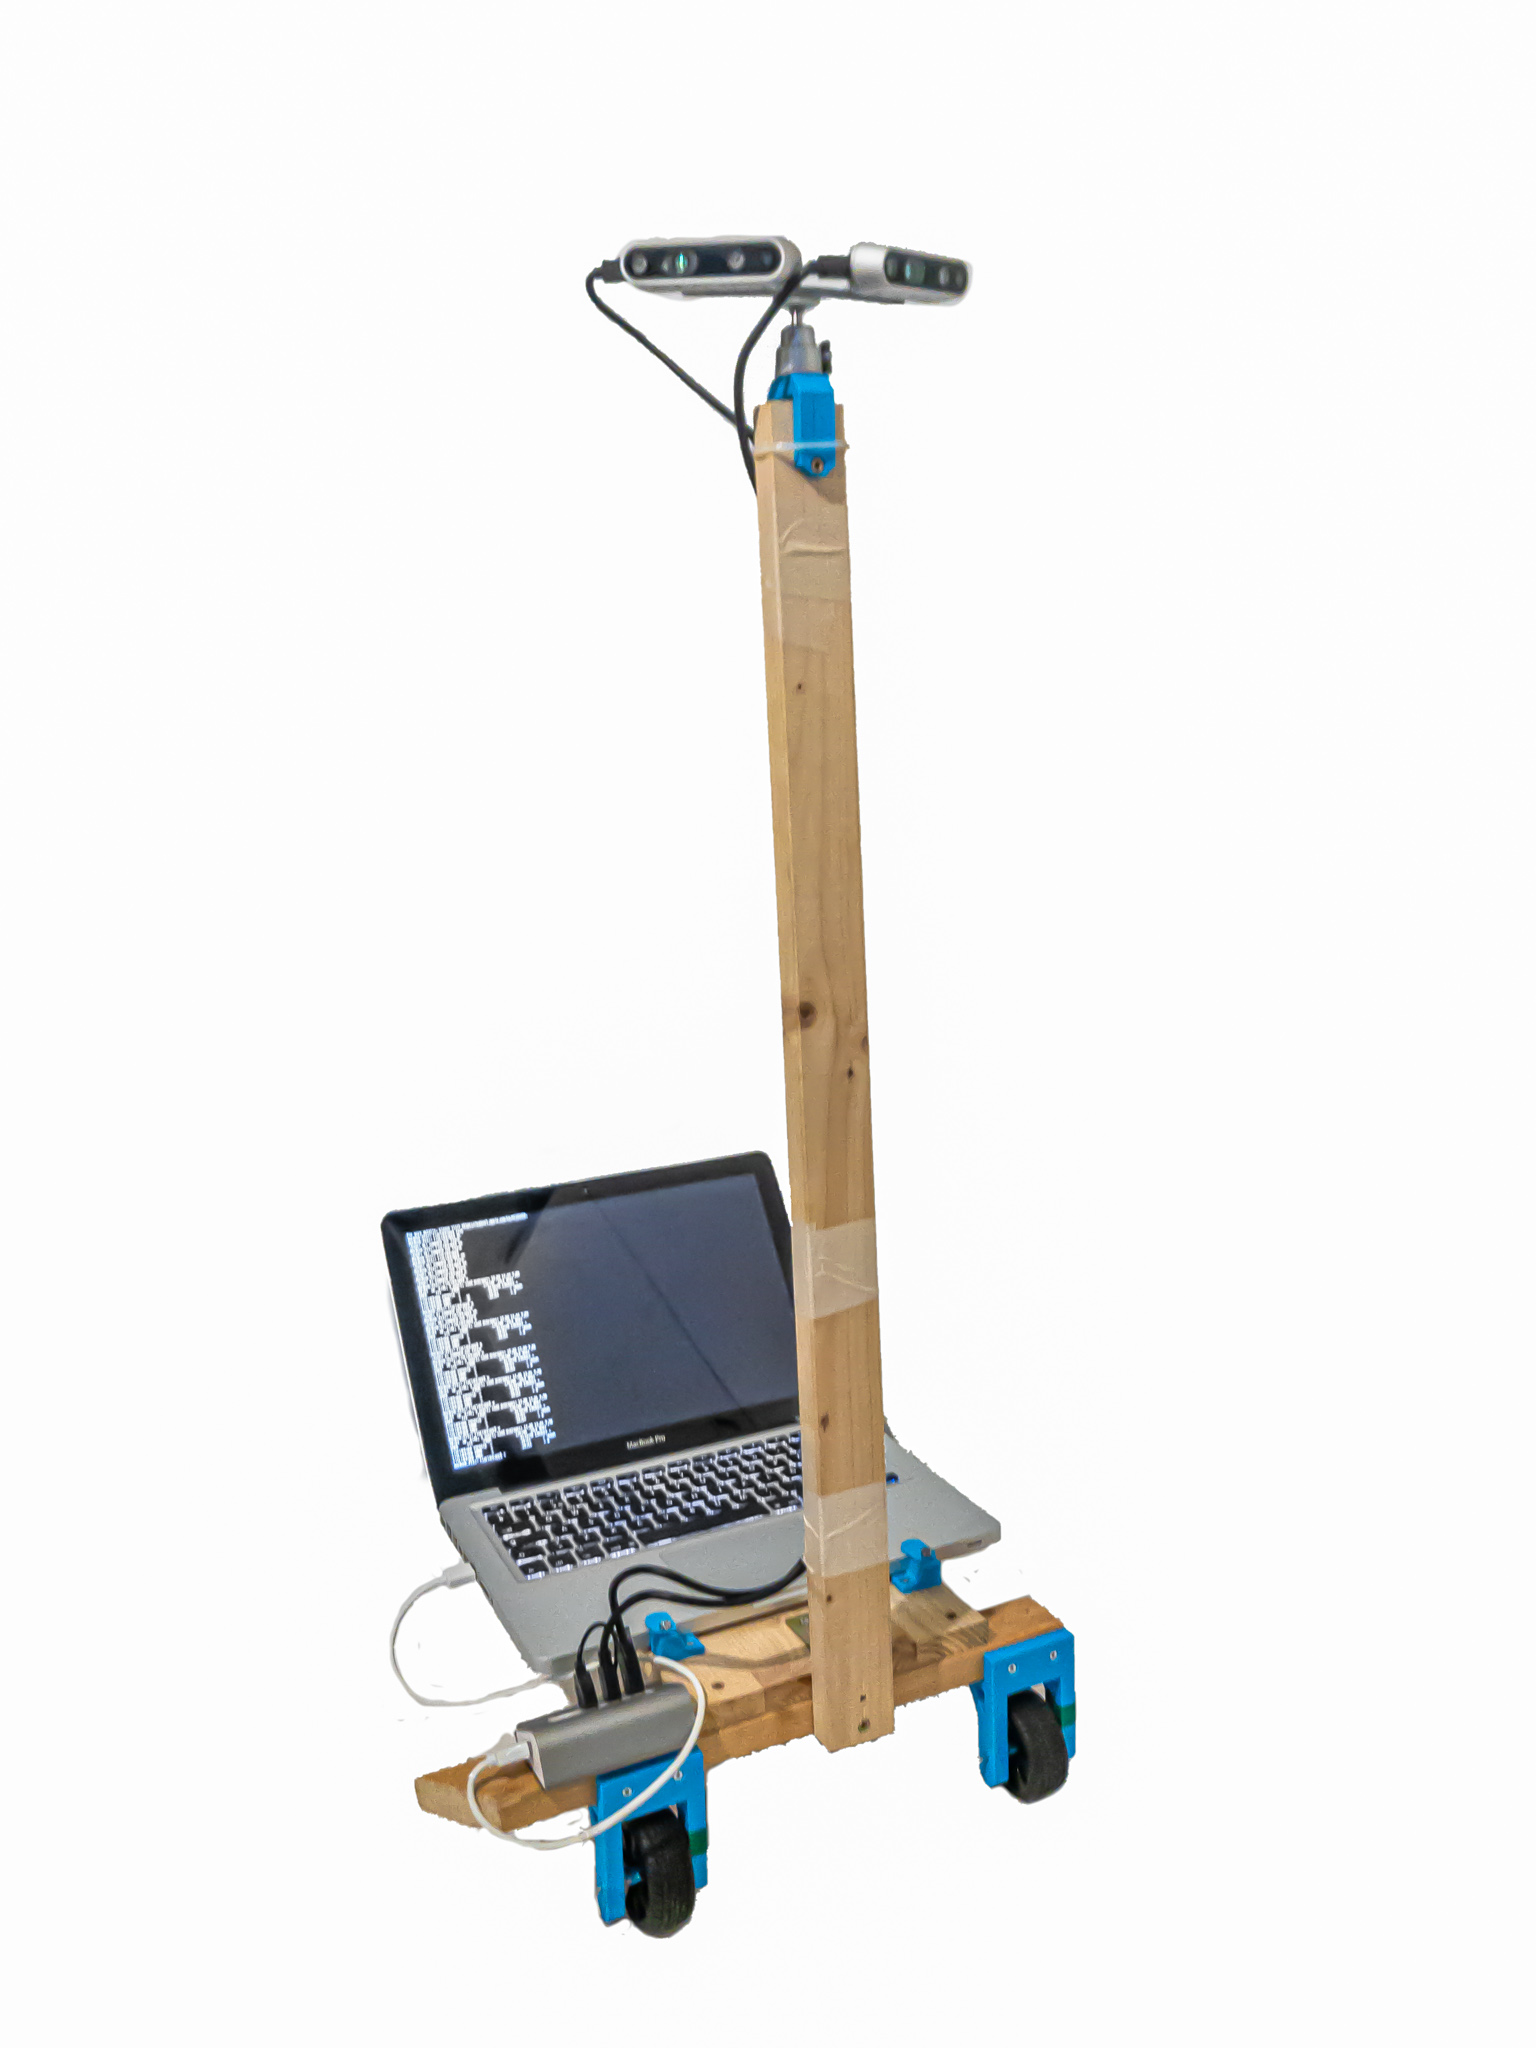
\includegraphics[width=\linewidth]{Bilder/laboter.jpg}
	\caption{Plattform für die Datenaufzeichnung }
	\label{fig:Laboter}
\end{minipage}
\hfill
 \begin{minipage}[t]{0.6\linewidth}
	\centering
	\includegraphics[width=\linewidth]{Bilder/Roboter_Differenzial_antrieb_2.png}
	\caption{Darstellung des Prinzips zur Ermittlung der neuen Pose }
	\label{fig:Odoemtrie}
\end{minipage}
\end{figure}

Die kostengünstigste und einfachste Lösung zur Erfassung von Odometrieinformationen stellen Drehgeber an den Rädern dar. Hierbei sind die Räder in 20 gleich große Kreisabschnitte aufgeteilt. Die Drehgeber erfassen, wie viele dieser Kreisabschnitte pro Rad durch die Rotation durchlaufen wurden. Aus der Anzahl der passierten Kreisabschnitte und dem Raddurchmesser kann die zurückgelegte Distanz eines Rads ermittelt werden. Hierbei sind nur die beiden Räder, die auf einer Achse liegen, mit Drehgebern ausgestattet, am Stützrad erfolgt keine Messung. Aus dem Abstand zwischen den beiden Rädern und den zurückgelegten Strecken pro Rad und pro Zeitschritt kann die Bewegung des Roboters ermittelt werden. Dies ist auf Abbildung \ref{fig:Odoemtrie} dargestellt. Die neue Posenschätzung ergibt sich durch folgende Gleichungen: 

\begin{subequations}
	\begin{align}
		\theta &= \theta + \dfrac{s_R-s_L}{l} \\
		x &= x + \dfrac{s_R+s_L}{2}*cos(\theta) \\
		y &= y + \dfrac{s_R+s_L}{2}*sin(\theta)
	\end{align}
\end{subequations}

Die Posenschätzungen werden mit einer Frequenz von 10 Hz ermittelt. Bei dieser Variante der Odometrieschätzung werden nur x,y,$\theta$-Posen geschätzt. Diese beschreiben die Lage im Raum in x,y-Richtung sowie den Winkel um die z-Achse. Da die Datensätze nur in Umgebungen auf ebenen Flächen aufgezeichnet wurden, ist diese Posenerfassung ausreichend.

Die Verarbeitung der Pulse, die die Inkrementalgeber erzeugen, übernimmt ein Arduino nano Mikrocontrollerboard auf Basis der ATmega328 MPU. Die Odometrieinformationen in Form von x,y,$\theta$-Posen werden auf dem Arduino berechnet und im ROS-Nachrichtenformat tf2/TFMessage gepuplished. Die Verbindung zum Rechner erfolgt über USB mit dem ROS-Bibliothek rosserial$\_$arduino \cite{rosserial2018}. 

Die Genauigkeit der erzeugten Odometrieinformation wurde überprüft, indem eine zuvor ausgemessene Strecke von etwa 40 m in Form eines U abgefahren wurde. Die Abweichungen betrugen sowohl in x- als auch in y-Richtung jedes Mal unter 1m. Diese Genauigkeit wurde als ausreichend für den angestrebten nutzen bewertet.

%Diese ist auf Abbildung \ref{fig:Test_Odometrie} dargestellt. Der Versuch wurde zehn Mal durchgeführt. Die aufgezeichneten Strecken wiesen dabei in x-Richtung eine Abweichung von etwa 20 cm auf. In y-Richtung betrugen die Abweichungen etwa. Die gesamt zurückgelegte Strecke variierte im Bereich von $\pm$60 cm. Diese Genauigkeit wurde als ausreichend für den angestrebten nutzen bewertet.

%\begin{figure}
%	\centering
%	\includegraphics[width=0.75\linewidth]{Bilder/Test_odometrie.png}
%	\caption{Test Genauigkeit der Odometrieinformationen}
%	\label{fig:Test_Odometrie}
%\end{figure}

\section[Ausstattung des Computers (Kopp)]{Ausstattung des Computers}

Für die Validierung des SegMap-Algorithmus wird eine Intel i7-7700 @ 3,6 GHz CPU sowie eine Nvidia Quadro P2000 GPU mit 5 GB Speicher verwendet. Außerdem stehen 16 GB DDR4 RAM zur Verfügung. Verwendet wurde das Betriebssystem Ubuntu 16.04 und die ROS-Version kinetic. Für das künstliche neuronale Netz wurde Tensorflow 1.8 genutzt. 

\section[Datensätze (Schmelzer)]{Datensätze}
\label{sec:Datensatz}

Zur Validierung des SegMap-Algorithmus werden indoor-Datensätze benötigt, die mit einer RGB-D Kamera erzeugt wurden. Außerdem werden Odometrieinformationen benötigt über die die ungefähre Pose des Roboters geschätzt werden kann. Die bereits erwähnten Anforderungen werden lediglich von SLAM-Datensätzen der TU München erfüllt. Daher wurden zusätzlich eigene Datensätze erstellt, um die Ergebnisse der Anwendung des Algorithmus umfassender analysieren zu können. Außerdem müssen ausreichend Trainingsdaten für das Training des Deskriptors erzeugt werden. 

Die verschiedenen Sensordaten werden in unterschiedlichen ROS-Sen\-sor\-nach\-rich\-ten\-for\-ma\-ten erwartet, die eine spezifische Datenstruktur vorgeben. Diese müssen auf teilweise vorgegebenen Topics gepublisht werden. 
%In ROS stellen Topics Busse dar, über die verschiedene Programmknoten Nachrichten austauschen. Hierbei ist jedoch fest definiert, welche Knoten senden und welche empfangen. 
Alle Nachrichten werden vom Algorithmus mit einer Rate von 10 Hz erwartet. Der Algorithmus lauscht auf vier verschiedene Nachrichten. Diese umfassen zum einen die Tiefeninformationen der Umgebungsabtastung im  sensor$\_$msgs/PointCloud2-Nachrichtenformat. Außerdem werden die Odometrieinformationen als Posenschätzung mit Zeitstempel in Form von geometry$\_$msgs/PoseStamped erwartet. Diese werden im Koordinatensystem der Roboterplattform angegeben, das auf dieser fest ist. Die Posenschätzung ist relativ zum Startpunkt des  Roboters, der den Ursprung des Odometrie-Koordinatensystems bildet. Daher wird zusätzlich zu jeder Posenschätzung die zugehörige Transformation vom Odometrie-Koordinatensystem zum Koordinanensystem der Roboterplattform mit demselben Zeitstempel benötigt, um eine Posenschätzung relativ zum Startpunkt des Roboters zu erhalten. Diese wird als Nachricht der Form geometry$\_$msgs/TransformStamped erwartet. Darüber hinaus werden alle Transformationen vom Odometrie-Ko\-or\-di\-na\-ten\-sys\-tem des Startpunkts der Odometrieaufzeichnungen bis zum Koordinanensystem der Kamera als tf2$\_$msgs/TFMessage benötigt. Tf2 ist eine ROS-Bibliothek für die Handhabung mehrere Transformationen. Es werden alle Beziehungen zwischen den Koordinatensystemen verfolgt und in einem Buffer ge\-spei\-chert. Alle Transformationen werden im /tf Topic gepublisht. Die Datensätze wurden alle in Form von bag-Dateien gespeichert. 
%Dies ist ein Dateiformat, in dem seriell ROS-Nachrichten in der Reihenfolge gespeichert werden, in der sie empfangen werden. Bei der Aufzeichnung wird für jedes Topic, dessen Nachrichten gespeichert werden sollen, ein Subscriber gestartet, der auf diese Nachrichten lauscht. Anschließend können die gespeicherten Nachrichten abgespielt werden, indem diese durch einen Publisher für andere Programmknoten veröffentlicht werden. Dadurch können die Sensornachrichten in ihrer genauen Zeitlichen Abfolge gespeichert werden und erscheinen dem Algorithmus beim abspielen, wie wenn die Nachrichten gerade von den Sensoren erzeugt wurden. 

\subsection[TUM Datensatz (Schmelzer)]{TUM Datensätze}
%https://vision.in.tum.de/data/datasets/rgbd-dataset

Die TU München stellt eine Sammlung von RGB-D Datensätzen für die Evaluierung visueller Odometrie und SLAM-Algorithmen frei zur Verfügung \cite{Sturm2012}. Verwendet wurden Datensätze der Kategorie Robot SLAM, die zusätzlich zu den RGB-D Daten auch Odometrieinformationen enthalten. Diese Datensätze wurden erstellt, indem eine Microsoft Kinect auf einem Pioneer Roboter montiert wurde. Dies ist eine kleine Roboterplattform, die in diesem Fall ferngesteuert wurde und die Odometriedaten aufgezeichnet hat. 

Die Tiefenbilder, die von der Microsoft Kinect erzeugt werden, haben eine Auflösung von 640$\times$480 Pixeln und werden mit einer Framerate von 30 Hz geliefert. Die Kamera verfügt über eine Reichweite von 4,5 m.

Die Datensätze wurden in einer Halle aufgezeichnet, in der durch verschiedene Objekte eine Umgebung aufgebaut wurde. Es wurden beispielsweise mehrere Trennwände aufgestellt und verschiedene andere Objekte um diese herum arrangiert, wie Stühle, Stative und ein Teddybär. 

So wurden drei verschiedene Datensätze aufgezeichnet, bei denen der Pioneer unterschiedlich durch die Umgebung navigiert wurde. Die Datensätze enthalten Schleifen, bei denen Teile des Roboterpfads mehrmals abgefahren wurden. 

Die Datensätzen können direkt in Form eines Bag-Files heruntergeladen werden. Da diese jedoch mit einer älteren ROS-Version aufgenommen wurden, mussten diese zunächst in das Formt der verwendeten ROS-Version migriert werden. Hierfür werden von ROS bereits Funktionen mitgeliefert, die dies umsetzen. Außerdem werden die Nachrichten mit einer viel zu hohen Framerate gepublisht. Daher werden alle auf 10 Hz heruntergesetzt. Die Tiefeninformationen liegen im Bag-File lediglich in Form eines Tiefenbildes im Nachrichtenformat sensor$\_$msgs/Image vor.Diese Nachrichten wurden mithilfe des mit ROS mitgelieferten depth$\_$image$\_$proc Nodes in eine Punktwolke umgewandelt. 

Die Odometrieinformtionen sind in den Transformationsnachrichten des Topics /tf enthalten. Diese werden von der ersten Transformation vom ortsfesten Odometrie-Koordinatnesystem zum Koordinatensystem der Roboterplattform gebildet. Um diese Nachrichten in die vom Algorithmus erwartete Form zu überführe, wird ein Subscriber erstellt, der auf die Transformationsnachrichten lauscht. Anschließend werden die Informationen dieser Nachrichten in die benötigten Formate geometry$\_$msgs/PoseStamped und geometry$\_$msgs/TransformStamped umgewandelt und erneut in zwei neuen Topics gepublisht. 

Wie bereits erwähnt, müssen alle Transformationen vom Odometrie-Ko\-or\-di\-na\-ten\-sys\-tem bis zum Kamera-Koordinatensystem, in dem die Tifeninformationen aufgenommen wurden, im /tf Topic gepublisht werden. Die Nachrichten sollten den gleichen Zeitstempel haben damit keine  Time-out Fehler bei der Verarbeitung der Informationen im Algorithmus auftreten. Daher wird ebenfalls der bereits erwähnte Subscriber auf die Transformation vom Odometrie-Koordinatensystem auf das Koordinatensystem der Roboterplattform verwendet. Sobald die Transformation empfangen wird, werden aus dem Transformationsbuffer die aktuellsten Transformationen zwischen den übrigen Koordinatensystemen bis zum kamerakoordinatensystem gelesen. Alle Transformationen werden gemeinsam  mit einer Rate von 10 Hz gepublisht. 

\begin{figure}
	\centering
	\includegraphics[width=\linewidth]{Bilder/TUM_Manipulation.png}
	\caption{Darstellung der Vorverarbeitung der Daten der TUM-Datensätze} 
	\label{fig:tum_manipulation}
\end{figure}

Abbildung \ref{fig:tum_manipulation} zeigt den Verlauf der Daten vom Bagfile, das die Nachrichten genauso speichert, wie sie erzeugt wurden, über die Manipulation bis sie in den SagMap-Algorithmus eingelesen werden können. Der Transformationssubscriber sowie die Publisher, die die verschiedenen Nachrichten die aus den Transformationen erzeugt werden veröffentlichen, werden in einem Node zusammengefasst. Mit Hilfe eines launch-Files kann dieser Node sowie der Node zur Erzeugung der Punktwolke gemeinsam gestartet werden. Dadurch werden direkt die vom Algorithmus erwarteten Nachrichten gepublisht und können von diesem weiterverarbeitet werden.  

\subsection[Eigener Datensatz (Schmelzer)]{Eigene Datensätze}

Die eigenen Datensätze wurden mit der vorgestellten Realsense D435 aufgenommen, die auf der Vorrichtung zur Odometire-Aufzeichnung montiert wurde. Hierbei befindet sich die Kamera auf einer Höhe von 85 cm über dem Boden. Die gewählten Umgebungen unterscheiden sich anhand ihrer Strukturen sowie der Anzahl und Größe der Objekte, die in diesen vorkommen. Es wurden verschiedene Wohnungsumgebungen aufgenommen, da diese  typischerweise wenig Freiflächen und viele Objekte enthalten. Außerdem wurden Daten in Büros aufgezeichnet. Diese enthalten ebenfalls wenig Freiflächen und ähnlich viele Objekte wie Wohnungen. Typischerweise treten jedoch viele gleiche Objekte auf, wie z.B. Schreibtische, Stühle und Computermonitore. Die Objekte stellen häufig Flächen dar. Zusätzlich wurden verschiedene Flurumgebungen aufgenommen.  Diese bestehen häufiger aus Freiflächen und enthalten vergleichsweise wenig Objekte. Daher könnte eine  zuverlässige Orientierung in diesen Umgebungen schwieriger sein. Alle Datensätze wurden so aufgezeichnet, dass gleiche Teile der Umgebungen mehrfach pro Durchlauf observiert werden. Es wurden sowohl Datensätzen mit als auch ohne Farbinformationen aufgezeichnet. Bei der Aufzeichnung der Datensätze mit der in Kapitel \ref{sec:stereo} vorgestellten Konfiguration mit zwei Kameras hat sich gezeigt, dass die zur Verfügung stehende Hardware zur Aufzeichnung der Datensätze nicht ausreichend ausgestattet ist, um die entstehende Datenmenge zu verarbeiten. Daher konnten leider keine verwertbaren Datensätze aufgezeichnet werden.
 
Die Realsense D435 Kamera kann mithilfe eines ROS Wrappers in das ROS-Framework eingebunden werden. Dieser enthält ein launch-File, das die Kamera so startet, dass die Daten direkt in ROS-Nachrichtenformaten gepublisht werden. Dieses launch-File wurde so angepasst, dass lediglich die Punktwolke sowie das Farbbild gepublisht werden. Die Punktwolke wird mit der benötigten Auflösung sowie im vorgegeben Punktwolkenformat übermittelt. Die kamera wird direkt so gestartet, dass die Nachrichten mit einer Framerate von 10 Hz gesendet werden, um nicht unnltig Bandbreite zu belegen. Dies ist besonders wichtig bei der in Kapitel \ref{sec:stereo} vorgestellten Konfiguration mit zwei Kameras. 

Die Odometrie-Vorrichtung veröffentlicht Transformationsnachrichten im tf2$\_$msgs/ TFMessage-Nachrichtenformat. Diese umfassen lediglich die  Transformationen vom Odometrie-Koordinatensystem zum Koordinatensystem der Odometrie-Plattform. In einem Publisher-Subscriber-Node, dessen Aufbau wie beim Manipulations-Node des TUM-Datensatzes ist, wird auf die Transformationsnachrichten gelauscht. Diese werden um die statische Transformation mit der angegebenen Höhe der Kamera vom Koordinatensystem der Odometrieplattform zu dem der Kamerabasis erweitert. Außerdem werden die Kamera-internen ROS-spezifischen Transformationen von der Kamerabasis bis zum Koordinatensystem, in dem die Punktwolke aufgenommen wurde, angehangen. Diese werden von der Kamera nach dem Start  einmal als statische Transformationsnachricht gepublisht. Da diese jedoch regelmäßig im /tf Topic in Verbindung mit dem gleichem Zeitstempel wie die anderen Transforamtionen benötigt werden, müssen diese jedes Mal erneut gepublisht werden. Im Subscriber werden also alle Transformationen zusammengefügt und dann gemeinsam im /tf Topic gepublisht. Die geometry$\_$msgs/PoseStamped und geometry$\_$msgs/TransformStamped Nachrichten werden wie bei der Manipulation der TUM-Datensätze erzeugt. 

\begin{figure}
	\centering
	\includegraphics[width=\linewidth]{Bilder/OLAF_Manipulation.png}
	\caption{Darstellung der Vorverarbeitung der Odometriedaten der eigenen Datensätze}
	\label{fig:olaf_manipulation}
\end{figure}

Abbildung \ref{fig:olaf_manipulation} zeigt den Verlauf der Daten von den Sensoren über die Ma\-ni\-pu\-la\-tion bis sie in den SagMap-Algorithmus eingelesen werden können. Wie beim TUM-Datensatz wurde ein launch-File erstellt, das den Publishe-Subscriber-Node zur Manipulation der Transformationsnachrichten sowie das launch-File der Kamera und der Odometrie startet. Dadurch werden direkt die Nachrichten gepublisht, die vom Algorithmus erwartet werden. 